\documentclass{amsart}
\usepackage{graphicx,float}
\usepackage{amsmath,xfrac,amssymb}
\usepackage{physics}
\usepackage{tikz}

 
\title{Quantum Field Theory Problem Sets}
\author{John Bortins}
 
\begin{document}
 
\maketitle{}


\section*{Notes}
Field operators create or annihilate particles at specific spatial locations. The second quantized single particle operator $\hat{A}=\sum_{\alpha\beta} \mathcal{A}_{\alpha\beta}\hat{a}^\dagger_\alpha \hat{a}_\beta $ is the sum over all processes which remove a single particle in state $\ket{\beta}$, multiply by $\mathcal{A}_{\alpha\beta}$, add a single particle in state $\ket{\alpha}$. Tight binding approximation. The second quantized two particle operator is $\hat{A}=\sum_{\alpha\beta\gamma\delta} \mathcal{A}_{\alpha\beta\gamma\delta}\hat{a}^\dagger_\alpha\hat{a}^\dagger_\beta \hat{a}_\gamma\hat{a}_\delta $. The Hubbard model is important to solid state physics.

\begin{figure}[H]
    \centering
    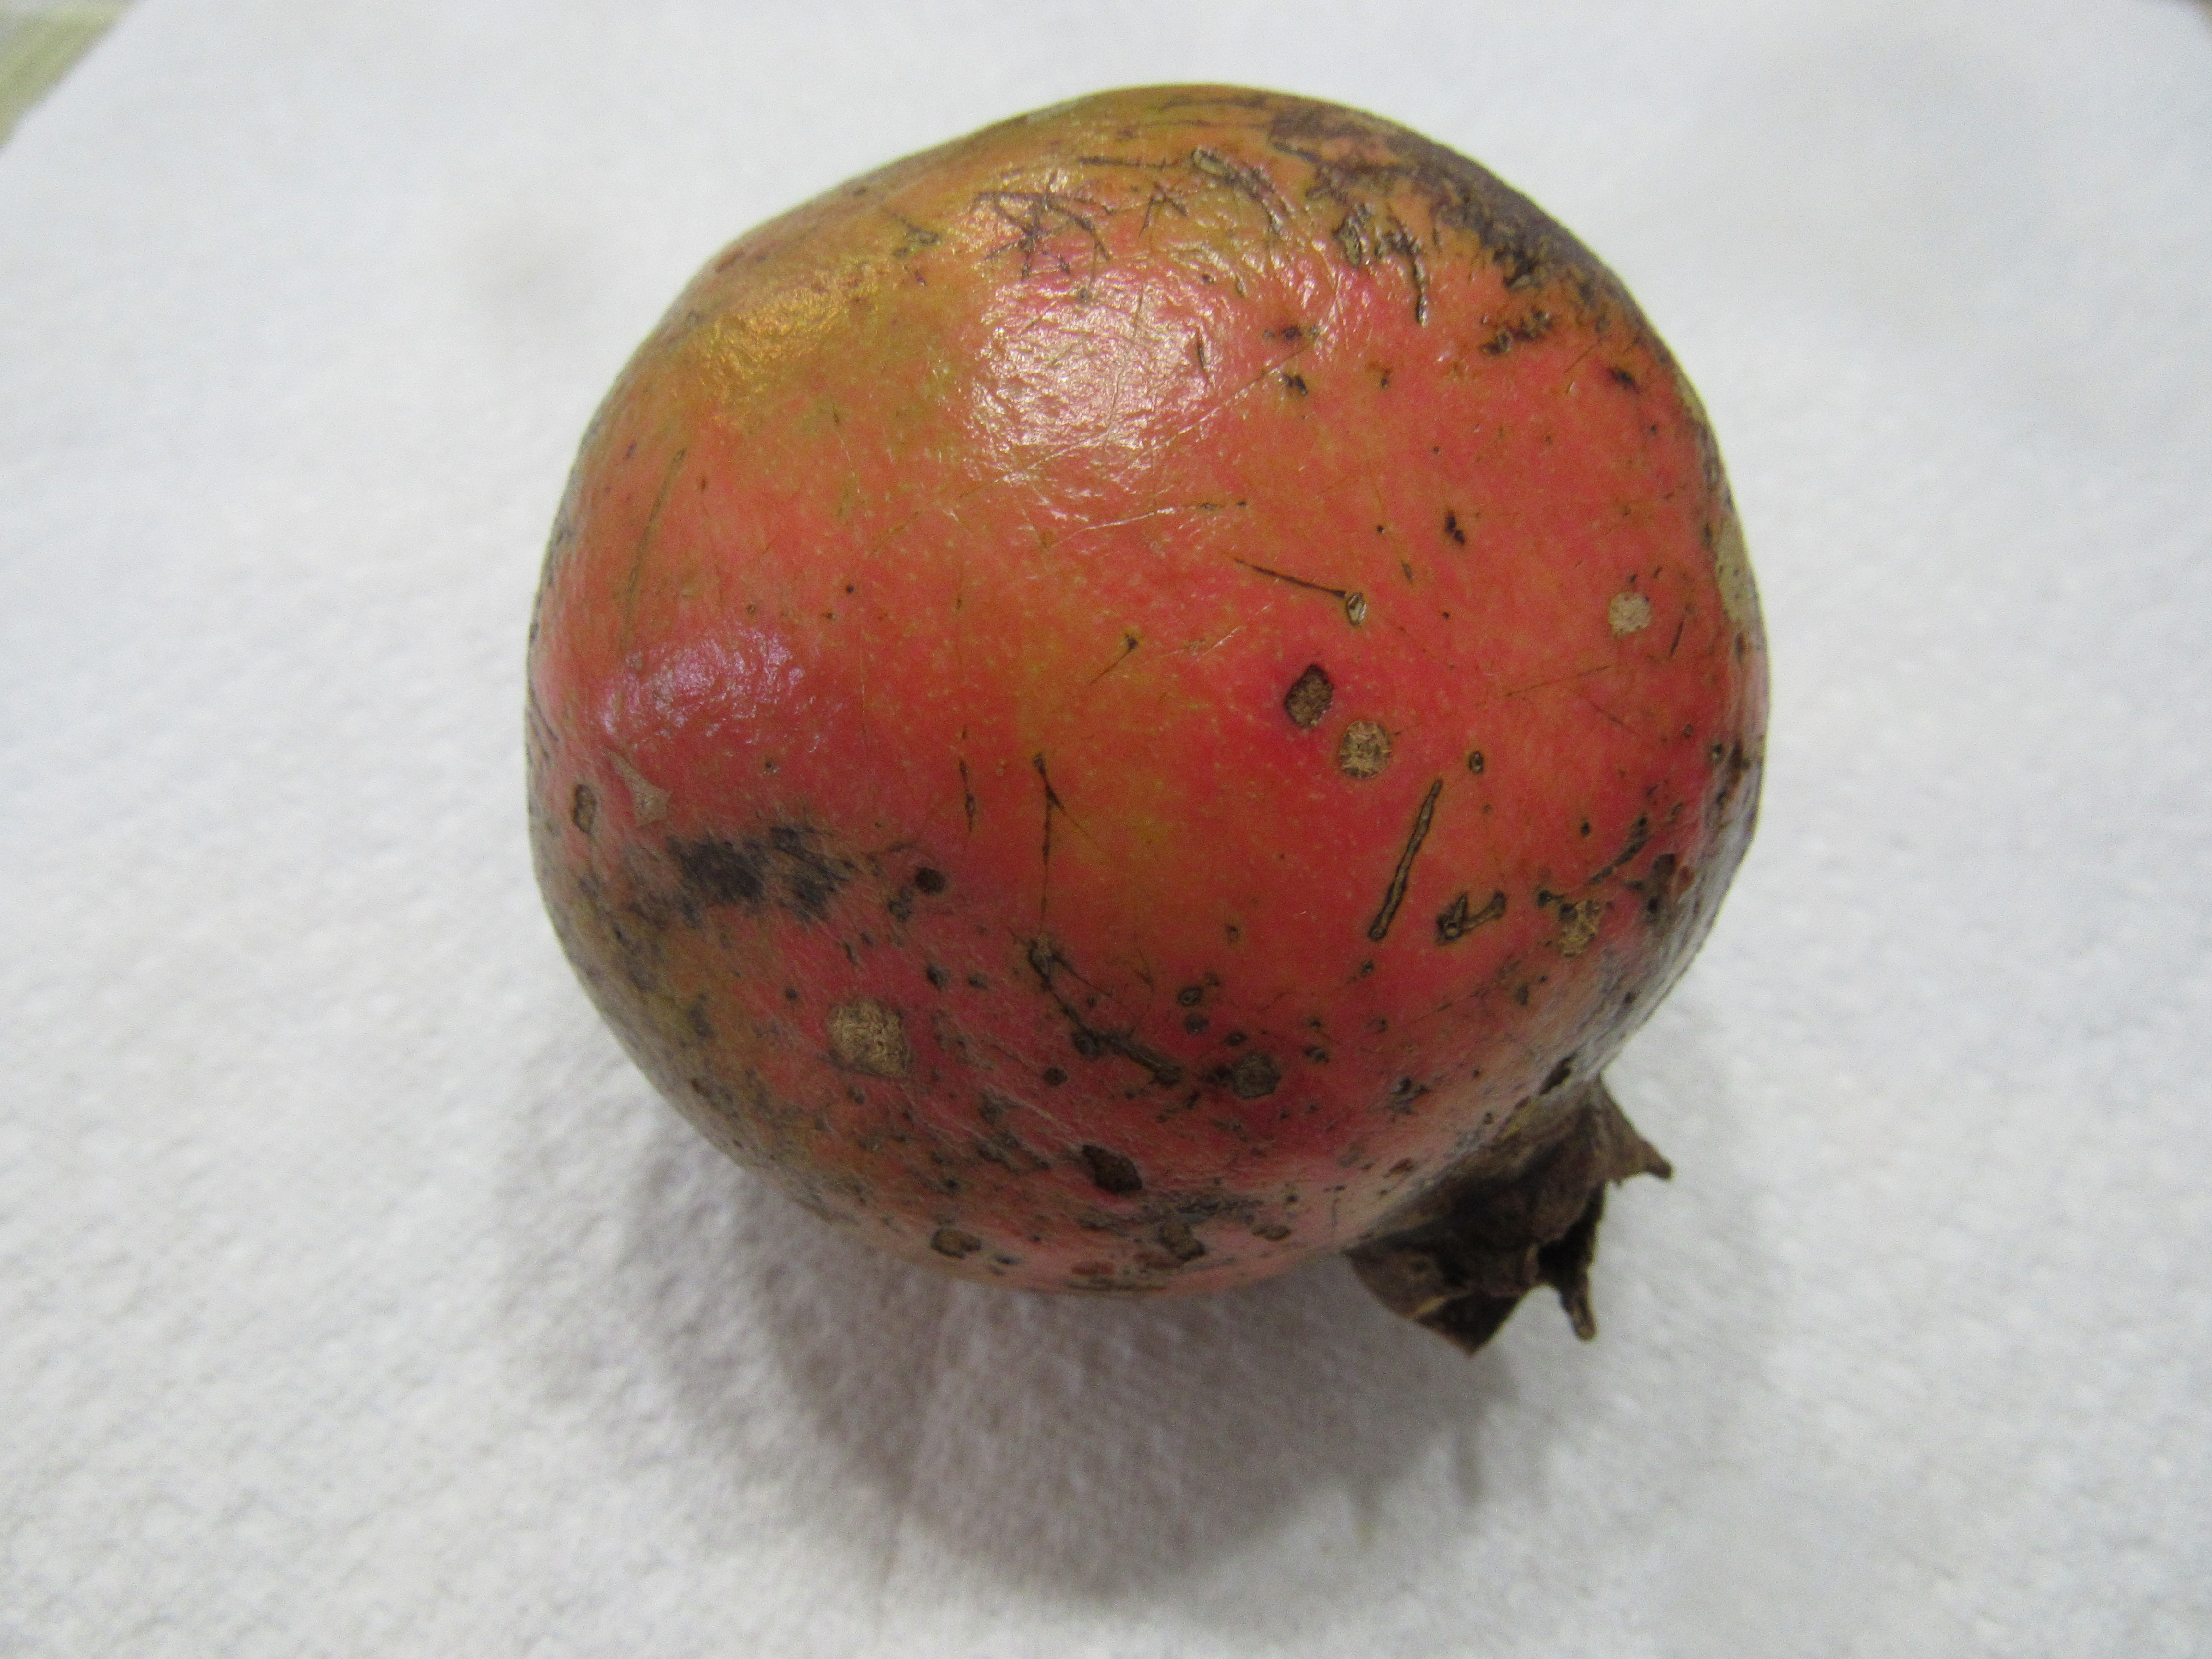
\includegraphics[width=0.5\textwidth]{IMG_0873}
    \caption{Pomegranate}
    \label{fig:awesome_image}
\end{figure}

\section*{Problem 4.1}
 
\[\qq*{Given} [\hat{A},\hat{B}]_{\zeta} = \hat{A}\hat{B}-\zeta\hat{B}\hat{A}\]

\[\text{For bosons}\qquad \zeta=1 \qquad[\hat{A},\hat{B}]_{\zeta} = [\hat{A},\hat{B}]\]

\[\text{For fermions}\qquad \zeta=-1 \qquad[\hat{A},\hat{B}]_{\zeta} = \{\hat{A},\hat{B}\}\]

The generalized commutation relations become

\[ [\hat{\psi}(\boldsymbol{x}),\hat{\psi}^\dagger(\boldsymbol{y})]_{\zeta} =\delta^{(3)}(\boldsymbol{x}-\boldsymbol{y})  \qquad\text{and}\qquad[\hat{\psi}(\boldsymbol{x}),\hat{\psi}(\boldsymbol{y})]_{\zeta} =0\]

\[ \text{Consider the operator}\qquad \hat{\rho}(\boldsymbol{x})\hat{\rho}(\boldsymbol{y})=
   \hat{\psi}^\dagger(\boldsymbol{x})\hat{\psi}(\boldsymbol{x})\hat{\psi}^\dagger(\boldsymbol{y})\hat{\psi}(\boldsymbol{y}) \]  

   From the first generalized commutation relation we get

\[  \hat{\psi}(\boldsymbol{x})\hat{\psi}^\dagger(\boldsymbol{y}) = \zeta \hat{\psi}^\dagger(\boldsymbol{y})\hat{\psi}(\boldsymbol{x})+\delta^{(3)}(\boldsymbol{x}-\boldsymbol{y})\]

\[ \text{Hence}\qquad \hat{\rho}(\boldsymbol{x})\hat{\rho}(\boldsymbol{y})=
    \zeta\hat{\psi}^\dagger(\boldsymbol{x})\hat{\psi}^\dagger(\boldsymbol{y})\hat{\psi}(\boldsymbol{x})\hat{\psi}(\boldsymbol{y})+
    \hat{\psi}^\dagger(\boldsymbol{x})\hat{\psi}(\boldsymbol{y})\delta^{(3)}(\boldsymbol{x}-\boldsymbol{y})\]  

From the second generalized commutation relation we get

\[  \hat{\psi}(\boldsymbol{x})\hat{\psi}(\boldsymbol{y}) = \zeta \hat{\psi}(\boldsymbol{y})\hat{\psi}(\boldsymbol{x})\]
 
\[ \text{Hence}\qquad \hat{\rho}(\boldsymbol{x})\hat{\rho}(\boldsymbol{y})=
   \zeta^2 \hat{\psi}^\dagger(\boldsymbol{x})
    \hat{\psi}^\dagger(\boldsymbol{y})\hat{\psi}(\boldsymbol{y})\hat{\psi}(\boldsymbol{x}) +\hat{\psi}^\dagger(\boldsymbol{x})\hat{\psi}(\boldsymbol{y})\delta^{(3)}(\boldsymbol{x}-\boldsymbol{y})\] 

\[\text{Clearly}\qquad \zeta^{2}=1 \]

\[ \hat{V}_{wrong} =\frac{1}{2 }\int \dd[3]{x}\dd[3]{y}V(\boldsymbol{x},\boldsymbol{y}) \hat{\rho}(\boldsymbol{x})\hat{\rho}(\boldsymbol{y}) \]

\[ \text{Hence}\qquad \hat{V}_{wrong} =\hat{V}+\frac{1}{2 }\int \dd[3]{x}V(\boldsymbol{x},\boldsymbol{x}) \hat{\psi}^\dagger(\boldsymbol{x})\hat{\psi}(\boldsymbol{x})\qquad\blacksquare
\]


\section*{Problem 4.2}

\[ \text{Define a single-particle density matrix by}\qquad  \hat{\rho}_{1}(\boldsymbol{x}-\boldsymbol{y})=\expval{\hat{\psi}^\dagger(\boldsymbol{x})\hat{\psi}(\boldsymbol{y})}\]

\[ {\psi}^\dagger(\boldsymbol{x})=\frac{1}{\sqrt{\mathcal{V}}} \sum_{\boldsymbol{q}} \hat{a}^{\dagger}_{\boldsymbol{q}}e^{-i\boldsymbol{q}\vdot\boldsymbol{x}} \qq{and}{\psi}(\boldsymbol{y})=\frac{1}{\sqrt{\mathcal{V}}} \sum_{\boldsymbol{p}} \hat{a}_{\boldsymbol{p}}e^{i\boldsymbol{p}\vdot\boldsymbol{y}} \]

\[ \expval{\hat{\psi}^\dagger(\boldsymbol{x})\hat{\psi}(\boldsymbol{y})}=
\expval{\qty(\frac{1}{\sqrt{\mathcal{V}}} \sum_{\boldsymbol{q}} \hat{a}^{\dagger}_{\boldsymbol{q}}e^{-i\boldsymbol{q}\vdot\boldsymbol{x}})\qty(\frac{1}{\sqrt{\mathcal{V}}} \sum_{\boldsymbol{p}} \hat{a}_{\boldsymbol{p}}e^{i\boldsymbol{p}\vdot\boldsymbol{y}} )} \]

\[ \expval{\hat{\psi}^\dagger(\boldsymbol{x})\hat{\psi}(\boldsymbol{y})}=
\frac{1}{\mathcal{V}}\sum_{\boldsymbol{pq}} \expval{ \hat{a}^{\dagger}_{\boldsymbol{q}}\hat{a}_{\boldsymbol{p}}e^{-i(\boldsymbol{q}\vdot\boldsymbol{x}-\boldsymbol{p}\vdot\boldsymbol{y})}} \qquad\blacksquare\]


\section*{Problem 4.3}

\[\text{For a general state}\qquad \ket{\psi}=a\ket{\uparrow\downarrow,0}+b\ket{\uparrow,\downarrow}+c\ket{\downarrow,\uparrow}+d\ket{0,\uparrow\downarrow} \]

\[\text{The Hubbard Hamiltionian is}\qquad \hat{H}=\mqty*(U&-t&t&0 \\-t&0&0&-t \\t&0&0&t \\0&-t&t&U) \]

Has eigenvalues $ \mqty(0,&U,&\frac{1}{2}\qty(U-\sqrt{16t^2+U^2}),&\frac{1}{2}\qty(U+\sqrt{16t^2+U^2})) $

(a) As $t\rightarrow0$, the eigenvalues go to $ \mqty(0,&U,&0,&U) \qquad\blacksquare$

(b) Extract U: $ \mqty(0,&U,&\frac{U}{2}\qty(1-\sqrt{\qty(\frac{4t}{U})^2+1}),&\frac{U}{2}\qty(1+\sqrt{\qty(\frac{4t}{U})^2+1})) $

For $0<\frac{t}{U}\ll 1$:  $ \mqty(0,&U,&\frac{U}{2}\qty(1-\frac{1}{2}\qty(\frac{4t}{U})^2-1),&\frac{U}{2}\qty(1+\frac{1}{2}\qty(\frac{4t}{U})^2+1)) $

Hence: $ \mqty(0,&U,&-\frac{4t^2}{U},&U+\frac{4t^2}{U}) \qquad\blacksquare$


\begin{align*}
\Pmqty{U&-t&t&0 \\-t&0&0&-t \\t&0&0&t \\0&-t&t&U}\Pmqty{a\\b\\c\\d}&=\lambda\Pmqty{a\\b\\c\\d}\\
\Pmqty{(U-\lambda)&-t&t&0 \\-t&-\lambda&0&-t \\t&0&-\lambda&t \\0&-t&t&(U-\lambda)}\Pmqty{a\\b\\c\\d}&=0\\
\end{align*}
Find the determinant using expansion by minors.
\begin{align*}
(U-\lambda)&[\lambda^2(U-\lambda)+\lambda t^2+\lambda t^2]+\\
t&[\lambda t(U-\lambda)-t^3+t^3]+\\
t&[t^3-t^3+\lambda t(U-\lambda)]+\\
0&=\determinant 0 \implies\\
\lambda^2(U-\lambda)^2+4\lambda t^2(U-\lambda)&=0\\
\lambda(U-\lambda)[\lambda(U-\lambda)+4t^2&=0
\end{align*}
Solutions are $\lambda=0$, $\lambda=U$, $\lambda^2 -U\lambda -4t^2=0$

\end{document}